\section{genetic Personalized Community Detection}

%
My proposed gPCD model contains an offline and an online step. Figure \ref{fig:pipeline} shows the pipeline of the whole framework. The offline step first encodes the user-independent binary community tree (\textit{Section \ref{sc:c3_offline}}), and subsequently learns embedding representations for both user need and nodes on the binary community tree (\textit{Section \ref{sc:c3_representation}}). The online step introduces the genetic personalized community detection approach (\textit{Section \ref{sc:c3_online}}). To accelerate the running speed, a distributed version of gPCD model is also deployed on HDFS (\textit{Section \ref{sc:c3_distributed}}).  To disambiguate the notations mentioned in this section to better explain the gPCD model, some commonly used notations can be found in Table \ref{tab:notation}. 

\subsection{Offline Community Tree Index} \label{sc:c3_offline}

One challenge of solving personalized community detection problem is the computational cost due to the complexity of personalization and graph structure. In order to reduce the online workload, most of computation cost is put into the one-time offline step whose time cost can be excluded from the online personalized community detection step. Thus, I first convert the graph into a binary community tree offline to retain user-independent community information. 

Infomap algorithm \cite{rosvall2011multilevel} is employed to generate the user-independent communities solely based on the graph \textit{G(V, E)}. Infomap algorithm simulates a random walker wandering on the graph and indexes the  description length of his / her random walk path via multilevel codebooks. By minimizing the description length based on the map equation below, community structures are formed for the graph.
%\begin{equation} \small
%\textit{$L(\mathcal{M})$} = q_{\curvearrowright}H(\mathcal{Q})+\sum_{i=1}^{m} \textit{$p_{\circlearrowright}^{i}$}H(\textit{$\mathcal{P}^{i}$}) 
%\end{equation}
%where $L(\mathcal{M})$ is the description length for a random walker in the current community $\mathcal{M}$. $q_{\curvearrowright}$ and $p_{\circlearrowright}^{i}$ are the jumping rates between communities and within the $i_{th}$ community. $H(\mathcal{Q})$ is the frequency-weighted average length of codewords in the global index codebook and $H(\mathcal{P}^{i})$ is frequency-weighted average length of codewords in the $i_{th}$ community codebook.

\begin{equation} 
\textit{$L(\pi)$} = \sum_{i}^{m}q_{\curvearrowright}^{i}H(\mathcal{Q})+\sum_{i=1}^{m} \textit{$p_{\circlearrowright}^{i}$}H(\textit{$\mathcal{P}^{i}$}) 
\end{equation}
where \textit{$L(\pi)$} is the description length for a random walker under current community partition $\pi$. $q_{\curvearrowright}^{i}$ and $p_{\circlearrowright}^{i}$ are the jumping rates between communities and within the $i_{th}$ community in each step. $H(\mathcal{Q})$ is the frequency-weighted average length of codewords in the global index codebook and $H(\mathcal{P}^{i})$ is frequency-weighted average length of codewords in the $i_{th}$ community codebook. Followed by this equation to partition communities into sub-communities , a hierarchical community tree \textit{$T_{c}(N^{c},L^{c})$} is constructed from the original graph $G(V,E)$. 
\begin{figure}  
	% \advance\leftskip-1cm  
	\center
	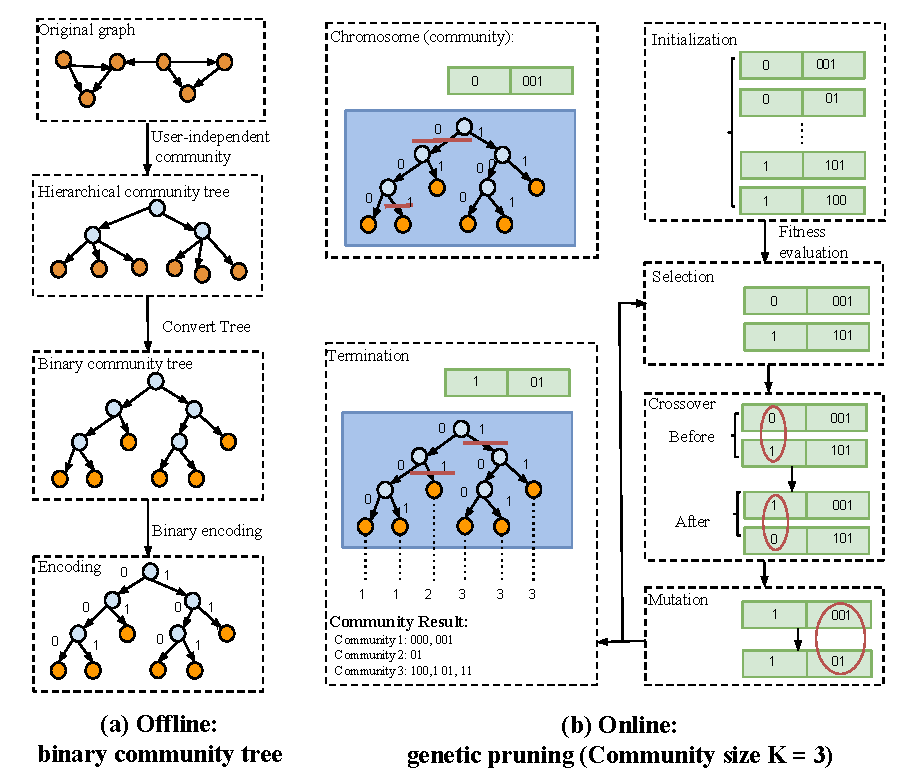
\includegraphics[width=1.0\columnwidth]{img/chapter3/4.pdf}
	%  \vspace{-3em}
	\caption{The framework of gPCD model. (a) refers to the offline construction step on the original graph and (b) refers to the online genetic pruning step to generate personalized communities.} 
	\label{fig:pipeline}
	%  \vspace{-1em} 
\end{figure}
In \textit{$T_{c}(N^{c},L^{c})$}, each parent node can have multiple child nodes which can be regarded as a community partition on the parent node. For instance, a node $N_{k}^{c} \in N^{c}$ from $T_{c}(N^{c},L^{c})$ represents a community of vertices.  Its $m$ child nodes $\{N_{k_{1}}^{c},N_{k_{2}}^{c},...,N_{k_{m}}^{c}\}$ represent $m$ sub-communities of vertices from $G(V,E)$ where we have $	\bigcap_{i=1}^{m} N_{k_{i}}^{c} = \varnothing$ and  $	\bigcup_{i=1}^{m} N_{k_{i}}^{c} =  N_{k}^{c}$.  



In order to achieve an efficient personalized community detection in the following online step, I convert the hierarchical community tree \textit{$T_{c}(N^{c},L^{c})$} to a binary community tree \textit{$T_{b}(N^{b},L^{b})$} for index. Specifically, for $m$ child nodes of a parent node $N_{k}^{c}$, a bottom-up approach is proposed to merge a selected pair of sibling nodes as a new node in an iterative manner. The approach runs until all $m$ child nodes merged together to form the parent node $N_{k}^{c}$. To avoid an unbalanced tree where small communities are always left to merge with huge communities in the end, I first select the node with the smallest community size among all sibling nodes in each merging step. It is merged with its sibling node with the largest normalized linked weight (Please refer to Figure \ref{fig:pipeline}(a)). The normalized linked weight function $w(\cdot)$ between  two nodes $N_{i}^{c}$ and $N_{j}^{c}$ is defined as:
\begin{equation} 
\textit{$w(N_{i}^{c},N_{j}^{c})$} =\frac{\textit{$N_{i}^{c}\odot N_{j}^{c}$}-\frac{\mathcal{D}(N_{i}^{c})\cdot \mathcal{D}(N_{j}^{c})}{2|E|} }{\textit{$| N_{i}^{c}||N_{j}^{c}|$}} 
\end{equation} 
where \textit{$N_{i}^{c}\odot N_{j}^{c}$} denotes the number of edges linked between vertices in node \textit{$N_{i}^{c}$} and \textit{$N_{j}^{c}$}, which can be interpreted as the linkage strength between them; \textit{$|N_{i}^{c}|$} is the number of vertices inside node \textit{$N_{i}^{c}$}; \textit{$\mathcal{D}(N_{i}^{c})$} is the out-degree of node \textit{$N_{i}^{c}$} (the total number of edges linked to other nodes) and \textit{$|E|$} is the total number of edges in the original graph $G(V,E)$ . $\frac{\mathcal{D}(N_{i}^{c})\cdot \mathcal{D}(N_{j}^{c})}{2|E|} $ denotes the random linkage strength between node \textit{$N_{i}^{c}$} and \textit{$N_{j}^{c}$}. The \textit{$w(\cdot)$} function calculates how much that two nodes are better connected beyond random connection and is normalized by node size. Given the node $N_{i}^{c}$ with the smallest community size and all its sibling node set $S$, The merging step can be formulated as:
\begin{equation}  
\begin{aligned} 
& N_{j}^{c} \Leftarrow \argmax_{N_{j}^{c} \in S}w(N_{i}^{c},N_{j}^{c})\\
& N_{*}^{c} = N_{i}^{c}\bigcup N_{j}^{c}
\end{aligned}
\end{equation}
The bottom-up process will stop until all child nodes are merged together to form the parent node. In the end, the hierarchical community tree \textit{$T_{c}(N^{c},L^{c})$} is fully converted to a binary community tree \textit{$T_{b}(N^{b},L^{b})$} with user-independent community information.  The node size $|N^{b}|$ as well as the link size $|L^{b}|$  in \textit{$T_{b}(N^{b},L^{b})$} is at most $2|V|$ which is smaller than the size of original graph $G(V,E)$. If I consider to form the binary community tree with only $k$ levels, the size of \textit{$T_{b}(N^{b},L^{b})$} can be even smaller. 

\begin{table}[h]
	%\scriptsize
	%	\small
	\centering
	
	\begin{tabular}{|p{3cm}|p{11cm}|} 
		\hline
		\textbf{Notations} & \textbf{Descriptions} \\ \hline
		$G(V,E)$ & Original graph $G$ with vertex set $V$ and edge set $E$ \\ \hline
		\textit{$T_{c}(N^{c},L^{c})$} & The hierarchical community tree generated from graph $G(V,E)$ with node set $N^{c}$ and link set $L^{c}$. Each node  $N^{c}_{k} \in N^{c}$ denotes a group of vertices belonging to $V$. \\\hline
		\textit{$T_{b}(N^{b},L^{b})$} & The binary community tree reconstructed from \textit{$T_{c}(N^{c},L^{c})$}. Each node $N^{b}_{k} \in N^{b}$ denotes a group of vertices belonging to $V$. \\ \hline
		$B$ & The binary codebook for \textit{$T_{b}(N^{b},L^{b})$}. Particularly, $B_{k} \in B$ denotes the binary code of both $N_{k}^{b} \in N^{b}$ and $L_{k}^{b}\in L^{b}$ where $L_{k}^{b}$ is the link points to node $N_{k}^{b}$.
		\\ \hline
	\end{tabular}
	\caption{Commonly used notations in gPCD model}
	\label{tab:notation}
	\vspace{-1em}
\end{table} 


For running time analysis, calculating normalized linked weight takes constant time. In each merging step, node pair selection takes linear time. Therefore, in the worst case, the time complexity of binary community tree construction is $O(|V|^2)$ where the depth of the hierarchical community tree $T_{c}(N^{c},L^{c})$ is 1 and each vertex in $G(V,E)$ forms a single-vertex community.

To encode the nodes and links on $T_{b}(N^{b},L^{b})$ as binary code, the root node is encoded as `null' first. For a parent node \textit{$N_{k}^{b}$} with its left child node \textit{$N^{b}_{k_{l}}$} and right child node \textit{$N^{b}_{k_{r}}$}, the binary code of a child node and the related link defined in the Notation Table \ref{tab:notation} is calculated as: 

\begin{eqnarray}\text{$B_{k_{i}}$}=
\begin{cases}
\text{$B_{k}$}+``0", & i = ``l"\cr 
\text{$B_{k}$}+``1", & i = ``r"
\end{cases}
\end{eqnarray} 

For instance, if the node \textit{$N_{k}^{b}$} is with binary code ``$00$," its left child node's binary code is ``$000$" while the right child node's binary code is ``$001$." The link \textit{$L_{k}^{b}$} that points to \textit{$N_{k}^{b}$} also has the binary code ``$00$". 

\subsection{Community and User Need Representation} \label{sc:c3_representation}

Node2vec \cite{grover2016node2vec} helps to learn fixed-length embeddings for both user need and communities. It simulates random walks on the graph $G(V,E)$ and learns the vertex embedding by optimizing the sequential relationships from random walk paths. In the end, each vertex $V_{k}$ in graph $G(V,E)$ has a vector representation as $\vec{V_k}$. Each node $N_{k}^{b}$ on the binary community tree \textit{$T_{b}(N^{b},L^{b})$} refers to a vertex community $C_{k}$ in the graph $G(V,E)$. Its representation $\vec{C_{k}}$ is calculated as the averaged embedding of all vertices inside the community. In the end, the binary community tree \textit{$T_{b}(N^{b},L^{b})$} represents the hierarchical community partition of Graph $G(V,E)$. Each node \textit{$N_{k}^{b}$} on the tree is indexed with three attributes: a group of vertices from graph $G(V,E)$, a binary code \textit{$B_{k}$}, and an embedding representation \textit{$\vec{C}_{k}$}.

On the other hand, User need (query) $I$ can also be represented by a combination of $t$ different vertices $\{V_1, V_2... V_t\}$ in the graph $G(V,E)$. In this study, two different scenarios for user need representation are offered:

\textbf{Vertex-based Query}. User need can be directly represented by the vertices based on the generation probability $P(V_k|I)$ between them. Hence the user need representation $\vec{I}$ is calculated as:

\begin{equation}
\vec{I} = \sum_{k=1}^{t} P(V_k|I) \cdot \vec{V_k} 
\end{equation} 
For instance, in a music sharing network, each vertex $V_k$ denotes a music and a user listing history can be used to reflect the user need $I$. $P(V_k|I)$ therefore can be regarded as the probability that a music being listened by the user. 

\textbf{Text-based Query}. Under this scenario, user need $I$ is represented as a text query, and each vertex $V_{k}$ in the graph $G(V,E)$ also contains textual content. From language model viewpoint, each vertex importance weight is the query likelihood $P(I|V_k)$, and the user need can is the weighted average of vertex embedding: 

\begin{equation}
\vec{I} = \frac{\sum_{k=1}^{t} P(I|V_k) \cdot \vec{V_k}}{\sum_{k=1}^{t} P(I|V_k)}
\end{equation}

In either case, user need is conceptualized as an embedding with the same dimension as the node embeddings on the binary community tree. It enables very efficient online personalized community detection in later steps. And running Node2vec takes most of the time in this step.   

\subsection{Online Genetic Pruning} \label{sc:c3_online}

The whole process, as the Figure \ref{fig:pipeline} shows, is to generate communities by pruning the constructed binary community tree. After each cut on a link, the original tree  will be separated into two sub-trees. After a specific number of cuts to the links on the tree, a fixed number of communities with different resolutions are detected.  By applying genetic selection, crossover, and mutation steps, the model converges to the optimized solution efficiently with a clear-defined fitness function. The details are shown in the following paragraphs.

\subsubsection{Genetic Representation} 

A chromosome is formed by a set of genes \{$g_{1},g_{2},...,g_{K-1}$\}, and each gene $g_{i}$ holds a cut link $L_{i}^{b}$ in the binary community tree \text{$T_{b}(N^{b},L^{b})$}. Since communities can be created by cutting links on the offline tree, a chromosome can be represented as a generated community partition of the original graph $G(V,E)$ in this way. 
To constrain a chromosome so that it can be decoded to a fixed number of communities, four \textbf{Cutting Rules} are necessarily to be applied: 
\begin{itemize} %\itemsep0em
	\item \textbf{ Rule 1}: If a link $L_{i}^{b}$ is picked to cut on the binary community tree \text{$T_{b}(N^{b},L^{b})$}, its pointing node $N_{i}^{b}$ will be retrieved and all the vertices within it form a community. 
	\item \textbf{ Rule 2}: If a link {$L_{i}^{b}$} and its ancestor link {$L_{j}^{b}$} are stored in the same chromosome, all vertices in {$L_{i}^{b}$}'s related node {$N_{i}^{b}$} are a subset of vertices in {$L_{j}^{b}$}'s related node {$N_{j}^{b}$}. In this case, the two cut links generate two communities where community $C_{i}$ is all vertices in $ N_{i}^{b}$ and community $C_{j}$ is the remaining vertices in $ N_{j}^{b}$ but not in $ N_{i}^{b}$. It can be formulated as   $C_{i} = \bigcup_{k}\{V_{k}|(V_{k}\in N_{i}^{b})\}$ and community $C_{j} = \bigcup_{k}\{V_{k}|(V_{k}\in N_{j}^{b}) \cap (V_{k}\notin N_{i}^{b})\}$.  
	\item \textbf{ Rule 3}: Sibling links can't be stored in the same chromosome, and it is not allowed to store duplicated links in a chromosome.
	\item \textbf{ Rule 4}: The depth's upper bound is set to be $d$, which means all eligible cut links should be located in the first $d$ depth on the binary community tree. It avoids to generate super tiny communities and hugely reduces the genetic searching scope on cut links.
\end{itemize} 

By applying the cutting rules to the online pruning process, I ensure a $K$ community partition can be retrieved from a chromosome with $K-1$ cut links.  


\subsubsection{Initialization}

Initially, the model generates a given number $P$  chromosomes as the seed ``chromosome population". And each iteration in the genetic approach breeds a new ``generation'' of chromosome population. In order to ensure a chromosome is an encoder of a $K$ community partition, $K-1$ links will be randomly picked (on the binary community tree) following the cutting rules and stored in the related genes of a chromosome. 

\subsubsection{Fitness Function} 

As each chromosome can be decoded as a community partition, it is important to measure the quality of each generated chromosome (how well the generated communities can satisfy user need). The measurement is hosted in a fitness function. 


In the proposed model, the fitness function simulates the user searching behavior on the graph given the community partition. For instance, a user can be more likely to pick the most relevant communities while avoiding the redundant information already selected. With the help of the offline step, the relevance score of node $N_{i}^{b}$ (community $C_{i}$) towards user need $I$ can be calculated with the cosine similarity $cos(\vec{I},\vec{C_{i}})$, and the information redundancy can be $\sum_{C_{j} \in S_c}cos(\vec{C_{j}},\vec{C_{i}})$ where $S_{c}$ is the set of communities that the user have already picked from the communities decoded from the target chromosome. Following this, I use a greedy selection approach to iteratively rank and pick communities given a chromosome (community partition) until all communities are picked: 

\begin{equation}  \argmax_{C_{i}}\lambda \cdot cos(\vec{I},\vec{C_{i}})-(1-\lambda)\cdot \frac{\sum_{C_{j} \in S_c}^{ }cos( \vec{C_j},\vec{C_{i}})}{|S_c|}
\end{equation} 

where $C_i$ is the candidate community to be picked and $|S_c|$ is the number of communities already been picked. $\lambda$ is a parameter controls  whether user prefers to obtain new useful information or to avoid redundant information.  

For chromosome quality evaluation, a query-generated vertex ranking list $l_{q}$ is first created by retrieving top $n$ vertices relevant to the query (user need) with the largest cosine similarities on embeddings of graph $G(V,E)$. I store the top $n$ vertex ranking label $R(l_{q})=\{1,2,...,n\}$ as the pseudo ground truth. On the other hand, given the $k_{th}$ chromosome $ch_k$ in the current chromosome generation, I can also retrieve the community-generated ranking of each vertex $V_{k} \in l_{q}$ from the sequentially selected communities decoded by the chromosome. I assign the ranking label on each vertex $V_{k}$ based on the following formula:
\begin{equation}
\sum_{V_{j} \in l_{q}}\Phi(\delta(V_{j}) < \delta(V_{k})) + 1
\end{equation} 

$V_{j}$ refers to all vertices in $l_{q}$. $\delta(V_{j})$ shows the ranking (selection sequence) of the community which $V_{j}$ belongs to. $\Phi$ is a binary operator to determine whether $V_{j}$ satisfy the condition $\delta(V_{j}) < \delta(V_{q})$. This formula helps to construct the community-generated ranking label $R(l_c)$. For instance, when $n=3$, I have a query-generated ranking list $l_q = \{V_1,V_2,V_3\}$ and its related ranking label $R(l_q) = \{1,2,3\}$. Given a chromosome where the community of $V_1$ and $V_2$ is the same and selected before $V_3$, I can generate the related community ranking label $R(l_c) = \{1,1,3\}$ with the same vertex sequence of $l_q$.

Then, I define the fitness function $f(\cdot)$ to evaluate the chromosome $ch_{k}$. As I have the query-generated ranking label $R(l_{q})$ (ground truth) and community-generated ranking label $R(l_{c})$ from $ch_{k}$, I calculate their Kendall's $\tau$  correlation coefficient  as the fitness score $f(ch_k)$ of chromosome $ch_k$ where higher score means the chromosome $ch_{k}$ can  generate better personalized communities to meet with user need. 

\begin{equation}
\textit{$f(ch_{k})$} = 1-\frac{\sum_{i=1}^{n} R(l_{ci})\cdot R(l_{qi})}{\sum_{i=1}^{n} R(l_{ci})^2\cdot \sum_{i=1}^{n}R(l_{qi})^2}
\end{equation} 
where $R(l_{ci})$ is the $i_{th}$ vertex ranking in community-generated ranking label $R(l_{c})$ and $R(l_{qi})$ is the $i_{th}$ vertex ranking in query-generated ranking label $R(l_{q})$. Kendall's $\tau$ is a widely used metric to evaluate the correlation between two lists where higher score means stronger correlation. Thus, higher fitness score reflects that the generated community ranking $R(l_{c})$ can better meet with user need $R(l_{q})$. 

Moreover, it is clear that the fitness function aims to separate all top $n$ vertices in different communities to get the optimal case. It matches the research goal to generate high resolution communities on vertices which are more relevant to user need. As the number of community is a given number $K$, it also leads to a coarser manner partition on the remaining less relevant vertices. On the other hand, the binary community tree $T_{b}(N^{b},L^{b})$ and the Cutting Rule 4 naturally preserve the community structure and unite the most relevant vertices in the same community. Hence the whole genetic approach is a gambling process. The final chromosome result is the equilibrium case to detect communities both contain graph topological structure and meet with user need.


\subsubsection{Selection}

I select the superior chromosomes from current chromosome population based on their fitness scores. The probability that the $k_{th}$ chromosome $ch_k$ is picked can be calculated via the Softmax normalization function $p(ch_{i}) = \frac{exp(f(ch_{k}))}{\sum_{i=1}^{P}exp(f(ch_{i}))}$. Then, the Fitness Proportionate Selection method is applied to randomly select $P$ chromosomes into chromosome pairs based on probability distribution. In order to enhance optimization efficiency, I also use elitism selection to ensure the best chromosome in the current generation will always be selected to the next generation. 

\subsubsection{Crossover} 

To reach global optimum community partition efficiently, given a pair of chromosomes, the crossover operation can randomly exchange part of the genes in both chromosomes to produce a new pair of chromosomes with a certain crossover rate.

In order to make sure that the newly generated chromosomes meet the cutting rules, an \textbf{Exchange Rule} is defined to restrict gene exchange: If gene \textit{$g$} contains link $L^{b}_{g}$, \textit{$g$} can't do crossover process with genes that contain either link $L^{b}_{g}$ or its sibling link $L^{b'}_{g}$. This rule can help avoid having duplicated links or sibling links stored together in the newly generated chromosome (To satisfy Cutting rule 3). 

After \textit{$m$} random numbers are selected from \{$1,2,...,K-1$\} as exchanged gene position indexes, genes located in the chosen positions of two chromosomes will exchange the stored link restricted by the Exchange Rule.
\subsubsection{Mutation} 
Mutation operation is applied to avoid local optimization. If a chromosome is chosen to mutate, a gene within the chromosome will be randomly picked, and its stored link will be changed to another link restricted by the Exchange Rules. An example is illustrated in Figure \ref{fig:pipeline}(b) where the link stored in the second gene is changed from ``001'' to ``01''. 

\subsubsection{Termination}

After $T$ iterations, the whole process stops and the current best chromosome is retrieved as the final result. Choosing the number of $T$ is dependent on the task. In order to decode the final chromosome to the related community partition, all genes in the chromosome are sorted in an ascending order based on the binary code of their stored cut link. Vertices whose binary codes start with the same cut link's binary code will be assigned to the same community label. And its later assigned community label can overwrite the previous assigned community label. For instance, if there are a vertex with binary code ``0011'' and two cut links with binary code ``00'' and ``001'', the vertex will be assigned to a community label ``00'' first, and its community label is overwritten by ``001'' afterwards. The Termination step in Figure \ref{fig:pipeline}(b) also illustrates a vivid example. In this way, the binary code of the binary community tree can help to decode the final chromosome into communities in an efficient way. 
 

\subsection{Distributed gPCD} \label{sc:c3_distributed}
 
To enhance the online step efficiency, a MapReduce framework is utilized to enable the distributed genetic evolution. Figure \ref{fig:distributed} depicts the personalized community detection under a MapReduce framework. The chromosome collection is either originally initialized from binary community tree or obtained from the last generation. It contains the whole chromosome population in the central depository. In its first ``Splitter'' process, all chromosomes are split into $M$ groups based on their hash values and sent out to related $M$  Mappers to calculate the ``Fitness'' scores. In the same Mapper, after all chromosomes are assigned fitness scores, based on their scores, a Combiner groups all chromosomes together and random select equal number of chromosomes with duplicated as the ``Selection'' step. All the selected chromosomes are sent to $R$ reducers (I set $R = M$ arbitrarily in order to better represent time complexity) to form pairs for the ``Crossover'' and  ``Mutation'' step, calculate new chromosome offsprings for the next generation and store them back to the central repository. 
 
\begin{figure}  
	% \advance\leftskip-4cm 
	\center
	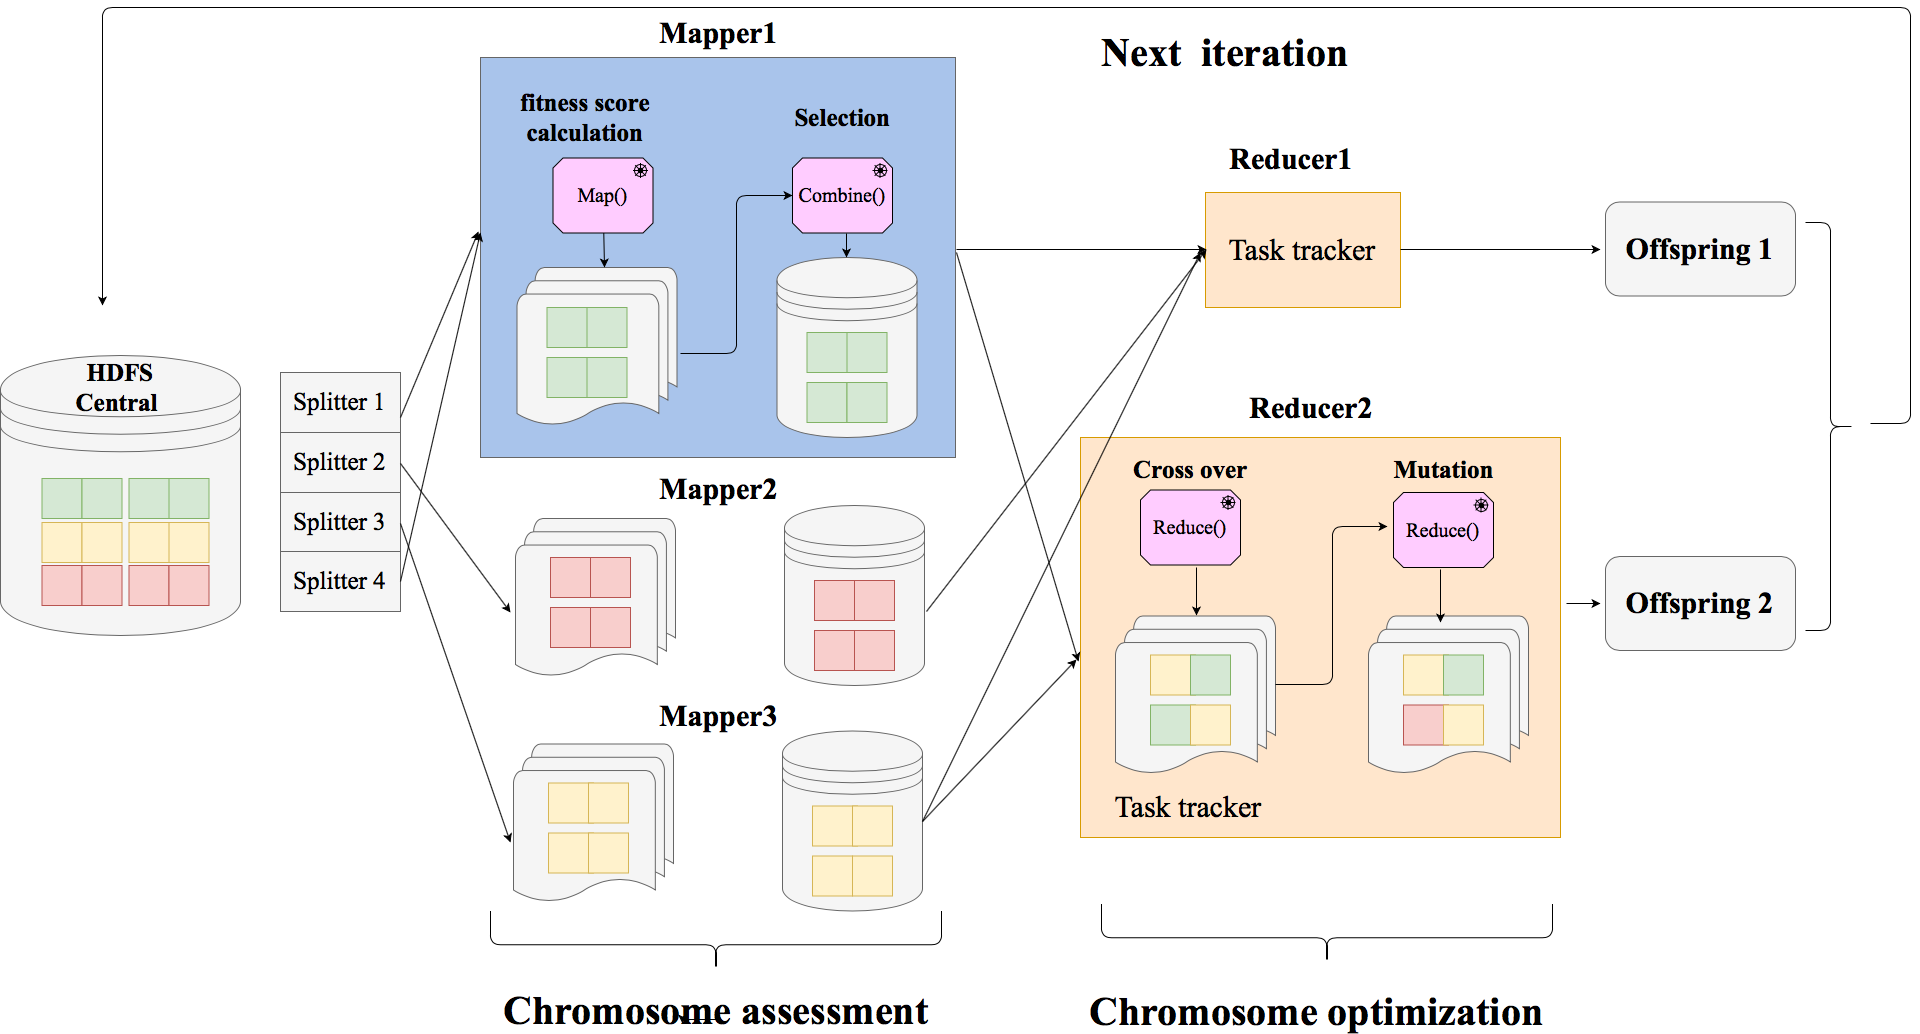
\includegraphics[width=1\columnwidth]{img/chapter3/parallel.png}
	%  \vspace{-3em}
	\caption{Online parallel computing process on Hadoop Distributed File System (HDFS)}
	%  \vspace{-1em} 
	\label{fig:distributed}
\end{figure}

The complexity of the proposed algorithm is $O(2^dKP)$ without parallel computing and $O(\frac{2^dKP}{M})$ with  parallel computing, where $d$ denotes the upper bound where the cut links are restricted in the top $d$ depth of the binary community tree $T_{b}(N^{b},L^{b})$; $K$ denotes the community number; $P$ denotes the initialized population size of the genetic algorithm and $M$ denotes the number of Mappers/Reducers in parallel environment. As all the parameters are considerably small (compared with the node/edge size in the original graph), the whole process runs very fast to retrieve the final community partition.